\section{Траектории землетрясений как смесь регрессий}
\subsection{Теория вариационного вывода}
Далее для смеси регрессий будет использоваться вариационной вывод~\cite{mean_field}. Кратко сформулируем и выпишем алгоритм вариационного вывода в общем виде

Пусть модель:

$$
p(X, Z, \theta) = p(X|Z)p(Z|\theta)p(\theta)
$$

Цель:
$$
p(Z,\theta|X) = \dfrac{p(X, Z, \theta)}{\int p(X, Z, \theta) dZd\theta}
$$

Самое сложное - это получить $\int p(X, Z, \theta) dZd\theta = p(X)$. Мы не можем вычислить $\int p(X, Z,\theta)dZd\theta$ напрямую. Тогда мы ограничиваем множество функций, в котором ищем решение как $q(Z,\theta) = q_z(Z)q_{\theta}(\theta)$. Такое ограничение называется "mean field approximation"

$$
\mathcal{F}(q) = \mathbb{E}_q  \log p(X,Z|\theta) + \mathbb{E}_q  \log p(\theta) - \mathbb{E}_q \log q(Z, \theta) = \\
= \mathbb{E}_q  \log p(X,Z|\theta) + \mathbb{E}_{q_{\theta}}  \log p(\theta) - \mathbb{E}_{q_{\theta}} \log q_{\theta}
(\theta) - \mathbb{E}_{q_{z}}  \log q_{z}(Z)
$$

Условия первого порядка:

$$
\dfrac{\delta}{\delta q_{\theta}}\mathcal{L} = \mathbb{E}_{q_{z}}
 \log p(X,Z|\theta) +  \log p(\theta) - ( \log q_{\theta}(\theta)+1) + \lambda_{\theta} = 0 
$$

$$
\dfrac{\delta}{\delta q_{z}}\mathcal{L} = \mathbb{E}_{q_{\theta}}
 \log p(X,Z|\theta) - ( \log q_{z}(Z)+1) + \lambda_z = 0 
$$

$$
\dfrac{\partial}{\partial \lambda_{\theta}}\mathcal{L} = \int q_{\theta}(\theta)d\theta - 1 = 0
$$

$$
\dfrac{\partial}{\partial \lambda_{z}}\mathcal{L} = \int q_{z}(Z)dZ - 1 = 0
$$

Тогда для $q_\theta$:

$$
q_{\theta}(\theta) = p(\theta) \mathbb{E}xp(\mathbb{E}_{q_{z}} \log p(X,Z|\theta)-1+\lambda_{\theta})
$$

$$
\lambda_{\theta} = 1 -  \log\int p(\theta) \mathbb{E}xp(\mathbb{E}_{q_{z}} \log p(X,Z|\theta)d\theta
$$

Окончательно

$$
q_{\theta}(\theta) = \dfrac{p(\theta) \mathbb{E}xp(\mathbb{E}_{q_{z}} \log p(X,Z|\theta))}{\int p(\theta) \mathbb{E}xp(\mathbb{E}_{q_{z}} \log p(X,Z|\theta)d\theta}
$$

В силу симметрии:

$$
q_{z}(Z) = \dfrac{ \mathbb{E}xp(\mathbb{E}_{q_{\theta}} \log p(X,Z|\theta))}{\int \mathbb{E}xp(\mathbb{E}_{q_{\theta}} \log p(X,Z|\theta)dZ}$$
\newpage

\subsection{Смесь регрессий}
\begin{itemize}
\item $D = \{(y_i, x_i)\}_{i=1}^N$
\item $y_i\in\mathbb{R},\text{ }x_i \in\mathbb{R^d}$
5\item Генеративная модель для y: $P(y_i|\theta) = \sum\limits_{k=1}^K\pi_k\mathcal{N}(y_i|x_i^T\beta_k, \tau_k)$ Т.е. мы моделируем $K$ независимых траекторий, каждая из которых описывается как $y_i = x_i^T\beta_k + \varepsilon_i^k$. Однако, мы не наблюдаем латентные переменные, поэтому $y$ описывается как смесь.
\item Введем латентные переменные принадлежности к кластеру $Z$ где для $z_n$ используется стандартная K-coding схема : $\{0;1\}^k$ and $\sum\limits_{k}z_nk = 1$ 
\item Для каждого $\beta_k$ введем нормальное априорное распределение $\mathcal{N}(\beta_k|\mu_{\beta}^0, \Sigma_0)$ и для $\tau_k$  Inverse-Gamma  $\text{IG}(\tau_k|a_0, b_0)$
\item  Мы хотим, чтобы число траекторий-кластеров определялось автоматически. Поэтому мы используем в качестве априорного распределения для весов разреженный Dirichlet distribution. Начиная с заведомого большего числа кластеров, итеративно мы сойдемся к k, $k << K$.
 \end{itemize}

Итак, модель:

$$
\prod\limits_{n=1}^N\prod\limits_{k=1}^K \left[\mathcal{N}(y_n|x_n^T\beta_k, \tau_k)\right]^{z_{nk}}\prod\limits_{n=1}^N\prod\limits_{k=1}^K\left[\pi_k\right]^{z_{nk}}
\text{Dir}(\pi |alpha_0)\prod\limits_{k=1}^K \mathcal{N}(\beta_k|\mu_{\beta_k}^0, \Sigma_0)\text{IG}(\tau_k|a_0, b_0)
$$

\subsection{Отличие от других подходов}
Рассмотрим несколько статей, рещающих такую же задачу разделения траекторий и укажем на отличия нашего решения. В качестве вывода мы использовали вариационный подход, получив решение в аналитическом виде. Также мы использовали априорные распределения на параметры модели в качестве регуляризации и для автоматического определения числа кластеров. В статьях же в основном используется MCMC семплинг, а для выбора числа кластеров информационный критерий.

\begin{itemize}
\item Dirichlet Prior + MCMC : "Estimating Mixtures of Regressions" Merrilee HURN , Ana JUSTEL , and Christian P. ROBERT~\cite{mix_one}
\item Dirichlet Process + MCMC: "Dirichlet Process Mixtures of Generalized Linear Models" Lauren A. Hannah, David M. Blei, Warren B. Powell~\cite{mix_two}
\item BIC критерий + EM алгоритм: "Extending the Akaike Information Criterion to Mixture Regression Models" Prasad A. NAIK, Peide SHI, and Chih-Ling T~\cite{mix_three}
 \end{itemize}

\subsection{Вероятностный вывод}
Будем строить вариационное приближение в классе плотностей, факторизующихся как:

$$
p(Z, \pi, \beta, \tau|D) = q(Z|X)q(\pi|X)q(\beta)q(\tau)
$$

Также, так как мы считаем, что выборка $iid$, то все распределения факторизуются по наблюдениям.

\subsubsection*{$q(\beta_k)$}

\begin{equation*}
\begin{aligned}
& \log q(\beta_k) \propto \mathbb{E}_{\setminus q(\beta_k)}\left[\sum\limits_{n=1}^N z_{nk}\log\mathcal{N}(y_n|x_n^T\beta_k,\tau_k)+\log\mathcal{N}(\beta_k|\mu_{\beta}^0, 
\Sigma_0)\right] = \\
& =  \mathbb{E}_{\setminus q(\beta_k)}\left[\sum\limits_{n=1}^N z_{nk}(-\frac{1}{2}\frac{1}{\tau_k}\left(y_n - x_n^T\beta_k)^T(y_n - x_n^T\beta_k)\right)-\frac{1}{2}(\beta_k - \mu_{\beta}^0)^T\Sigma_0^{-1}(\beta_k - \mu_{\beta}^0)\right] = \\
&  = \mathbb{E}_{\setminus q(\beta_k)}\left[(Y-X\beta_k)^T\text{diag}(\dfrac{z_{nk}}{\tau_k})(Y-X\beta_k) - \frac{1}{2}(\beta_k - \mu_{\beta}^0)^T\Sigma_0^{-1}(\beta_k - \mu_{\beta}^0)\right] = \\
& = -\frac{1}{2}(Y - X\beta_k)^T W_k (Y-X\beta_k) - \frac{1}{2}(\beta_k - \mu_{\beta}^0)^T\Sigma^{-1}_0(\beta_k - \mu_{\beta}^0), \\
& \text{where }W_k = \text{diag}\left(\dfrac{\mathbb{E}_{q(z)} z_{nk}}{\mathbb{E}_{q(\tau)}\tau_k}\right)
 \end{aligned}
 \end{equation*}  

Поэтому, $q(\beta_k)\sim\mathcal{N}(\beta_k|\mu_{\beta}^k, \Sigma_k)$. Чтобы найти параметры, мы максимизируем квадратичную форму, также используем $q(\tau, z)=q(z)q(\tau)$

\begin{equation*}
\begin{aligned}
& Q(\beta_k) =  -\frac{1}{2}(Y - X\beta_k)^T W_k (Y-X\beta_k) - \frac{1}{2}(\beta_k - \mu_{\beta}^0)^T\Sigma^{-1}_0(\beta_k - \mu_{\beta}^0) \\
& \nabla Q(\beta_k) = -\left(X^TW_k(X\beta_k - Y)+\Sigma^{-1}_0(\beta_k - \mu_{\beta}^0)\right) = 0 \\
& \beta_k^{*} = \mu_{\beta}^k = \left(XW_k X + \Sigma_0^{-1}\right)^{-1}\left[X^TY + \Sigma^{-1}_0 \mu_{\beta}^0  \right] \\
& W_k = \left(XW_k X + \Sigma_0^{-1}\right)^{-1} \\
& \text{where }W_k = \text{diag}\left(\dfrac{\mathbb{E}_{q(z)} z_{nk}}{\mathbb{E}_{q(\tau)}\tau_k}\right)
 \end{aligned}
 \end{equation*}  

\subsubsection*{$q(\tau_k)$}

\begin{equation*}
\begin{aligned}
& \log q(\tau_k) \propto \mathbb{E}_{\setminus q(\tau_k)}\left[\sum\limits_{n=1}^N z_{nk}\left(-\frac{n}{2}\log \tau_k - \frac{1}{2}\frac{1}{\tau_k}(y_n - x_n^T\beta_k)^T(y_n - x_n^T\beta_k)\right) -(a_0 + 1)\log\tau_k - \frac{b_0}{\tau_k} \right] = \\
& = - \left(\frac{n}{2}\sum\limits_{n=1}^N \mathbb{E}_{q(z)}z_{nk} + a_0 + 1\right)\log\tau_k - \frac{1}{2}\frac{1}{\tau_k}\left(b_0 + \sum\limits_{n=1}^N \mathbb{E}_{q(z, \beta)}z_{nk}(y_n - x_n^T\beta_k)^T(y_n - x_n^T\beta_k)\right)
 \end{aligned}
 \end{equation*} 

Отсюда $q(\tau_k)\sim\text{IG}(\tau_k|a_k, b_k)$. Используя $q(z,\beta)=q(z)q(\beta)$:

\begin{equation*}
\begin{aligned}
& a_k = a_0 + \frac{n}{2}\sum\limits_{n=1}^{N}\mathbb{E}_{q(z)}z_{nk} \\
& b_k = b_0 +  \sum\limits_{n=1}^N \mathbb{E}_{q(z,\beta)}z_{nk}(y_n - x_n^T\beta_k)^T(y_n - x_n^T\beta_k) \\
& \sum\limits_{n=1}^N \mathbb{E}_{q(z,\beta)}z_{nk}(y_n - x_n^T\beta_k)^T(y_n - x_n^T\beta_k) = \text{Tr}\left(Z_k\mathbb{E}_{q(\beta)}(Y-X\beta)(Y-X\beta)^T\right), \text{ where } Z_k = \text{diag}\left(\mathbb{E}_{q(Z)}z_{nk}\right) \\
& \text{, finally: } \\
& b_k = b_0 + \frac{1}{2}\left[\left(Y - X\mu_{q(\beta_k)}\right)^TZ\left(Y - X\mu_{q(\beta_k)}\right)\right] + \frac{1}{2}\text{Tr}\left(X^TZX\Sigma_{q(\beta_k)}\right)
 \end{aligned}
 \end{equation*} 

\subsubsection*{$q(Z)$}

\begin{equation*}
\begin{aligned}
& \log q(z) \propto \mathbb{E}_{\setminus z}\sum\limits_{n=1}^N\sum\limits_{k=1}^K z_{nk}\left[\log\mathcal{N}(y_n|x_n^T\beta_k, \tau_k) + \log \pi_k\right] \\
& \mathbb{E}z_{nk} = \rho_{nk} \\
& \log\rho_{nk} = \mathbb{E}_{\setminus z}\sum\limits_{n=1}^N\sum\limits_{k=1}^K z_{nk}\left[\log\mathcal{N}(y_n|x_n^T\beta_k, \tau_k) + \log \pi_k\right] = \\
& = \mathbb{E}_{q(\pi)}\log\pi_k - \frac{1}{2}\log 2\pi - \frac{1}{2}\mathbb{E}_{q(\tau_k)}\log\tau_k - \mathbb{E}_{q(\tau_k)}\tau_k^{-1}\left((y_n-x_n^T\mu_{q(\beta_k)}x_n^T)^2 + x_n^T\Sigma_{q(\beta_k)}x_n\right)
 \end{aligned} 
 \end{equation*}

\subsubsection*{$q(\pi)$}
\begin{equation*}
\begin{aligned}
& \log q(\pi) \propto \mathbb{E}_{\setminus \pi}\sum\limits_{n=1}^N\sum\limits_{k=1}^K z_{nk} \log\pi_k + \log \text{Dir}
 \end{aligned} 
 \end{equation*}

Так что, $q(\pi)\sim\text{Dir}(\pi|\alpha_0 + \sum\limits_{n=1}^N\mathbb{E}_{q(z)}z_{nk})$

Все необходимые матожидания это матожидания достаточных статистик распределений из экспоненциального класса и легко выписываются.
\newpage

\subsection{Иллюстративные примеры на исскуственных данных }
Так как вариационный алгоритм сходится к локальному максимому, мы делаем несколько запусков и выбираем тот, который получил наибольшую ELBO.

Примеры, показывающие разделение траекторий:

\begin{figure}[H]
   \centering
   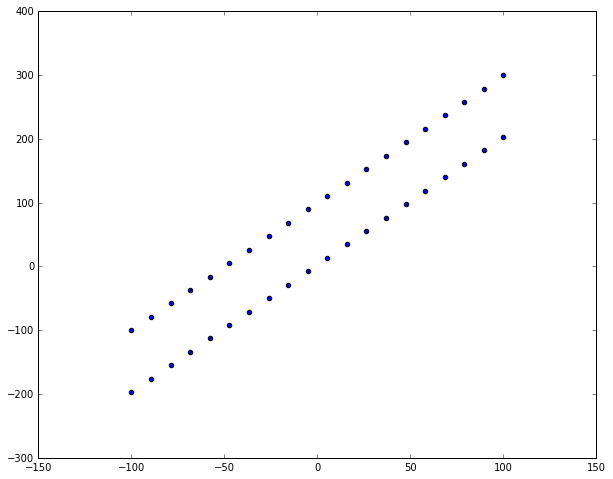
\includegraphics[scale=0.15]{figures/two_ground_truth.png}
   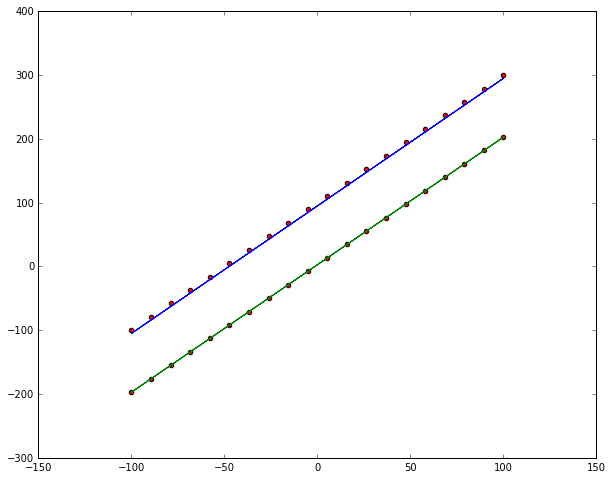
\includegraphics[scale=0.15]{figures/two_result.png}
 \end{figure}

Second example, ground truth and model work MAP estimation of regression:
\begin{figure}[H]
   \centering
   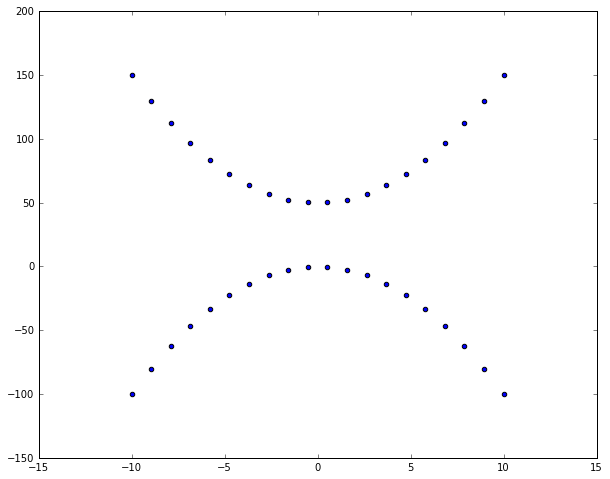
\includegraphics[scale=0.15]{figures/parabals_ground_trough.png}
   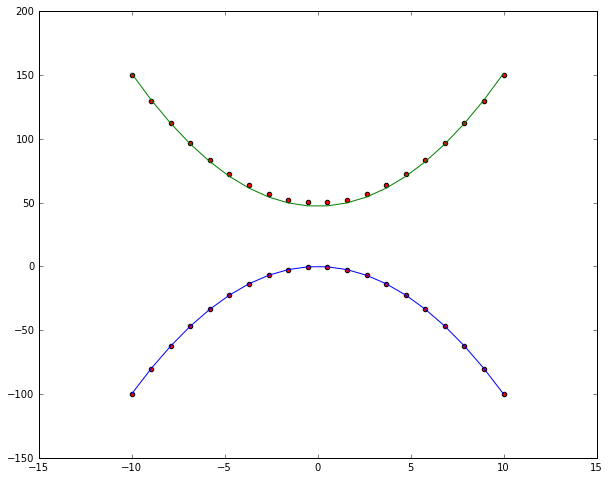
\includegraphics[scale=0.15]{figures/parabals_mixture.png}
 \end{figure}

Пример, показывающий автоматический подбор числа кластеров:
Старутем с  $K=24$ кластеров, и Dirichlet prior $\alpha_0^k = 0.1,~\forall k$. Сходимся к 3 кластерам, что соотвествует механизму генерации данных.

\begin{figure}[H]
   \centering
   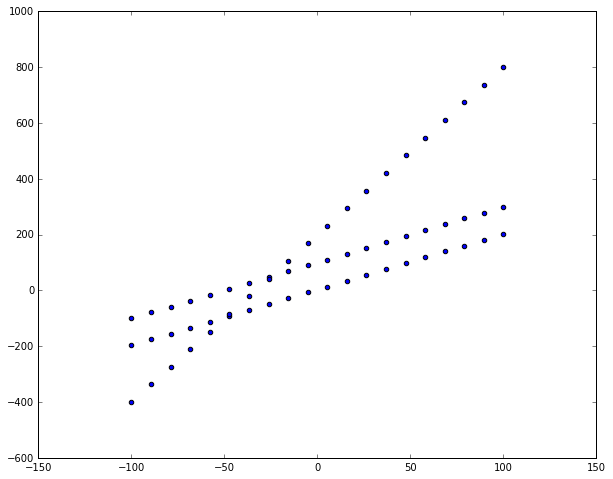
\includegraphics[scale=0.15]{figures/cross_ground_truth.png} 
   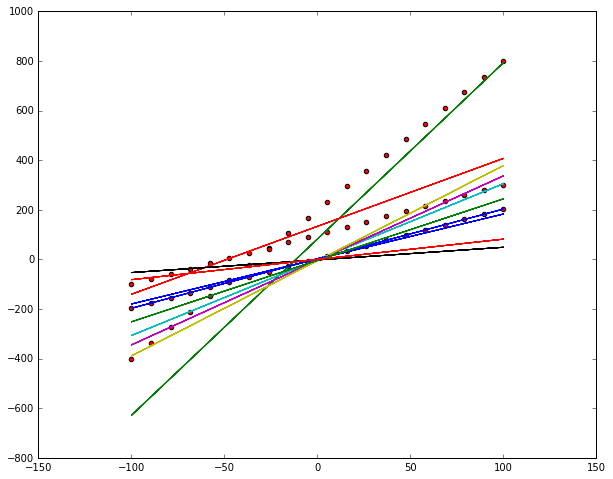
\includegraphics[scale=0.15]{figures/first_iter_cross.png}
   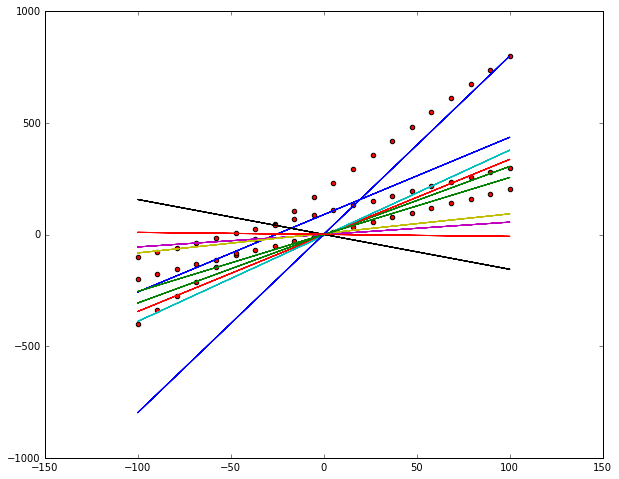
\includegraphics[scale=0.15]{figures/second_iter_cross.png}
   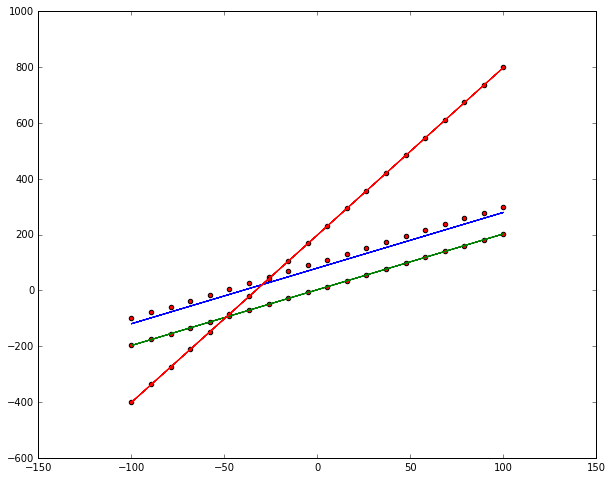
\includegraphics[scale=0.15]{figures/final_iter_cross.png}
 \end{figure}
\newpage

\subsection{Кластеризация вдоль траектории}
Также мы можем кластеризовать данные вдоль траекторий. Рассмотрим модельные примеры. В каждом из них обычная смесь гауссиан дает избыточное число кластеров по сравнению с кластеризацией вдоль траекторий.

Один пример:

\begin{figure}[H]
    \centering
    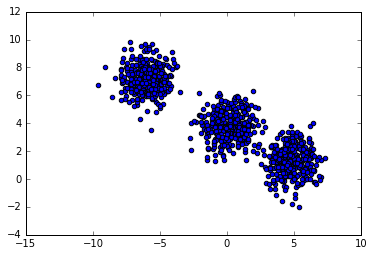
\includegraphics[scale=0.35]{figures/unsupervised_linear.png} 
    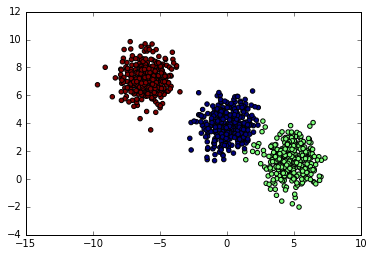
\includegraphics[scale=0.35]{figures/unsupervised_gmm.png}
    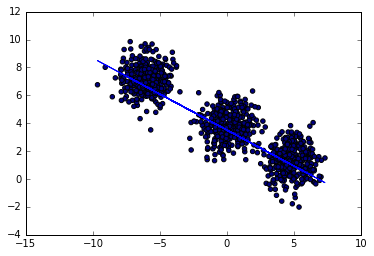
\includegraphics[scale=0.35]{figures/unsupervised_clustering.png}
   \end{figure}

Другой пример:

\begin{figure}[H]
    \centering
    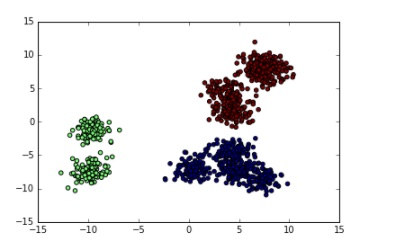
\includegraphics[scale=0.35]{figures/gaussian_mixture.jpg}
    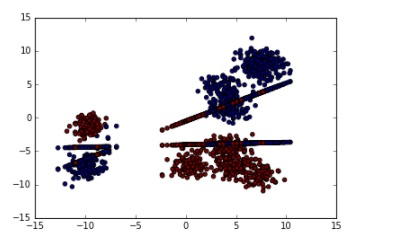
\includegraphics[scale=0.35]{figures/linear_regression_mixture.jpg}
   \end{figure}

\subsection{Использование для предсказания землетрясений}
\begin{itemize}

\item Декластеризация каталогов землетрясений
Как было отмеченно ранее (в секции про b-value прекурсор) многие рассматриваемые в литературе прекурсоры землетрясений опираются на предпосылку о пуассоновском распределении землетрясений в каталоге. В тоже время это противоречит природе землетрясений: они кластеризуются в результате фошоков и афтершоков.  Чтобы исправить ситуацию, нужно выделить такие последовательности и удалить все наблюдения, кроме одного, с наибольшей магнитудой. Как метод выделений таких последовательность можно использовать предложенную процедуру кластеризации вдоль направлений.

\item Выявление типичных траекторий и рассчет статистик внутри них
Однако мы поступим иначе и не будем удалять наблюдения. Вместо этого рассчитаем такие направления по месячным подвыборкам и будем рассчитывать прекурсоры в таких кластерах. 
\end{itemize}
